\section{Σκοπός διαμορφωτικού σχεδιασμού}

Το στάδιο του προκαταρκτικού σχεδιασμού αποτελούσε τη θεμελίωση του εγχειρήματος, όπου πραγματοποιήθηκε η δόμηση της κεντρικής ιδέας και ο καθορισμός των βασικών αρχών λειτουργίας του ρομπότ. Σε εκείνο το στάδιο, ο στόχος δεν ήταν η λεπτομέρεια, αλλά η απόδειξη της σκοπιμότητας της λύσης. Οι υπολογισμοί που εκπονήθηκαν είχαν χαρακτήρα εκτίμησης της τάξης μεγέθους, στοχεύοντας να αποδείξουν ότι η προτεινόμενη αρχιτεκτονική είναι φυσικά και τεχνικά υλοποιήσιμη.

\par Πλέον, ακολουθεί το στάδιο του διαμορφωτικού σχεδιασμού, το οποίο αποτελεί τη γέφυρα μεταξύ της θεωρητικής σύλληψης και της κατασκευαστικής πραγματικότητας. Σε αυτή τη φάση, η αρχική ιδέα μετουσιώνεται σε μια πλήρως ορισμένη μηχανολογική οντότητα. Οι προσεγγιστικές τιμές του προηγούμενου σταδίου αντικαθίστανται από ακριβείς διαστάσεις και αυστηρές ανοχές, καθώς εκπονούνται λεπτομερή κατασκευαστικά σχέδια και τρισδιάστατα μοντέλα (CAD). Παράλληλα, οι μαθηματικοί υπολογισμοί παύουν να είναι διερευνητικοί και γίνονται επιβεβαιωτικοί: στόχος είναι η πλήρης εξακρίβωση της μηχανικής αντοχής και της αξιοπιστίας της κατασκευής υπό τις πραγματικές συνθήκες φόρτισης που θα αντιμετωπίσει στο πεδίο. Μέσω αυτής της διαδικασίας, διασφαλίζεται ότι το τελικό σύστημα δεν είναι απλώς μια λειτουργική ιδέα, αλλά μια στιβαρή κατασκευή ικανή να ανταπεξέλθει στις απαιτήσεις της αποστολής διάσωσης.

\par Στην παρόν έρευνα, όπως έχει ήδη αναφερθεί, ο ολοκληρωμένος διαμορφωτικός σχεδιασμός αποτελεί έναν στόχο με χρονική διάρκεια ολοκλήρωσης πολύ μεγαλύτερη της επιθυμητής. Επομένως, καθώς ξεφεύγει των ενδιαφερόντων της παρόν εργασίας, θα πραγματοποιηθούν μετρημένες μελέτες των μηχανολογικών εξαρτημάτων για τη παρουσίαση μιας πιο ολοκληρωμένης σχεδιομελέτης. Στη πραγματικότητα, κατά αυτό το στάδιο, πρέπει να ορισθούν επακριβώς, η αρχιτεκτονική και το λειτουργικό σύστημα της πλατφόρμας, καθιστόντας την ικανή να ανταπεξέλθει τις συνθήκες μιας αποστολής διάσωσης. Ωστόσο, οι στόχοι του διαμορφωτικού σχεδιασμού στο παρόν πλαίσιο θα είναι:
\begin{itemize}
    \item Η ανάλυση της οδοντοκίνησης, τόσο γεωμετρικά όσο και λειτουργικά, για τις οδοντοκινήσεις του βραχίονα και της ερπύστριας. Θα ορισθεί επακριβώς η γεωμετρία των οδοντώσεων και θα εκλεθούν οι συντελεστές ασφαλείας της εφαρμογής.
    \item Η ανάλυση της λειτουργικότητας των μηχανολογικών εξαρτημάτων του συστήματος κίνησης. Θα αναλυθούν επακριβώς οι τρόποι με τους οποίους, τα επιλεγμένα μηχανολογικά εξαρτήματα λειτουργούν στην πλατφόρμα.
    \item Η ανάλυση των εδράνων κύλισης όσο αναφορά την αντοχή των εδράσεων. Θα αναλυθούν λειτουργικά οι εδράσεις των ατράκτων των ατέρμονων κοχλιοειδών τροχών. Οι περαιτέρω εδράσεις δεν θα αναλυθούν με βάση την αντοχή τους. 
    \item Η επεξήγηση της επικοινωνίας της πλατφόρμας με το σταθμό τηλεχειρισμού και η πρόταση μιας λύσης που ικανοποιεί τις απαιτήσεις της αποστολής.
\end{itemize}

Να σημειωθεί ότι, οι οδονοτοκινήσεις θα επιλυθούν αρχικά γεωμετρικά, και έπειτα θα ορισθούν κατάλληλα για να ικανοποιούν επαρκείς συντελεστές ασφαλείας. Τα έδρανα κύλισης δε θα αναλυθούν όλα, καθώς η επίλυση όλων των εδράσεων θεωρείται ότι ξεφεύγει του χρονικού πλαισίου εκπόνησης της παρόν εργασίας. Επομένως, για εξακρίβωση και ορθή υλοποίηση όλου του συστήματος της οδοντοκίνησης, επιλέγεται να επιλυθούν τουλάχιστον οι εδράσεις στο συγκεκριμένο υποσύστημα.



\section{Ανάλυση μηχανολογικών στοιχείων}
\subsection{Ανάλυση οδοντωτών τροχών}
% worm gear pair
Όπως έχει ήδη αναλυθεί και σε προηγούμενα κεφάλαια, μερικά βασικά γεωμετρικά στοιχεία των οδοντοκινήσεων ήταν απαραίτητο να ορισθούν πριν το στάδιο του διαμορφωτικού σχεδιασμού για την επιλογή των κινητήρων της πλατφόρμας. Αυτά τα στοιχεία φαίνονται στον \ref{tab:calcTorque}. Με βάση αυτά θα πρέπει να υπολογιστούν και μερικά ακόμη γεωμετρικά χαρακτηριστικά. Αυτά θα υπολογσιτούν τόσο για την οδοντοκίνηση της ερπύστριας όσο και του βραχίονα. Στη συνέχεια, σε παρακάτω κεφάλαια, θα εισαχθούν τα μεγέθη αυτά στο λογισμικό υπολογισμού αντοχής γραναζιών KISSsoft 2025 Student Version. Παρακάτω παρατηρούνται μερικά βασικά γεωμετρικά μεγέθη.
\begin{figure}[H]
    \centering
    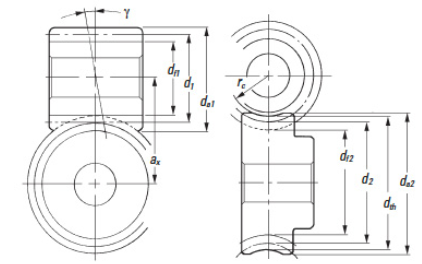
\includegraphics[width=0.5\linewidth]{media/khkDim.png}
    \caption{Γεωμτρικές διαστάσεις οδοντοκίνησης ατέρμονα - τροχού \cite{khk}.}
    \label{fig:khkDim}
\end{figure}
\par Αρχικά πρέπει να υπολογιστεί το αξονικό μέτρο οδόντωσης. Αυτό, σύμφωνα με τις αναλυτικές σχέσεις της αναφοράς \cite{handbook} προκύπτει:


% 1. Αξονικό Μέτρο (Axial Modulus)
\begin{equation}
    m_x = \frac{p_x}{\pi}
\end{equation}


Έπειτα, πρέπει να υπολογιστεί το ύψος της κεφαλής του δοντιού. Αυτό είναι:


% 2. Ύψος Κεφαλής (Addendum)
\begin{equation}
    a = 0.3183 \cdot p_x
\end{equation}


Ο οδοντωτός τροχός σε μια οδοντοκίνηση ατέρμονα - τροχού, κατεργάζεται με ακτίνα καμπυλότητας κατά το μήκος του δοντιού για τη σωστή εφαρμογή του με τον ατέρμονα. Η ακτίνα αυτή προκύπτει με βάση τη διάμετρο λειτουργίας του ατέρμονα όπως δίνεται στην αναφορά \cite{khk} καθώς το βιβλίο των Shigley J. κ.ά. δεν αναγράφει κάποια αναλυτική σχέση για τον υπολογισμό της. Έτσι υπολογίζεται επίσης και η διάμετρος του λαιμού του γραναζιού:
% 3. Ακτίνα Λαιμού Κορώνας (Throat Radius of Gear) -khk
\begin{equation}
    r_c = \frac{D_W}{2} - a
\end{equation}

% 5. Διάμετρος Λαιμού Κορώνας (Gear Throat Diameter)
\begin{equation}
    D_{t,g} = D_G + 2 \cdot a
\end{equation}

Στη συνέχεια υπολογίζεται το ενεργό ύψος της οδόντωσης:
% 4. Ενεργό Ύψος Οδόντωσης (Working Depth)
\begin{equation}
    h_k = 0.6366 \cdot p_x
\end{equation}

Χρειάζεται να υπολογιστούν και τα πλάτη των οδοντωτών τροχών. Για τον ατέρμονα υπολογίζεται το ελάχιστο μήκος του. Το μήκος δηλαδή που κατεργάζεται η οδόντωση στην άτρακτο του:

% 6. Ελάχιστο Μήκος Ατέρμονα (Minimum Facewidth of Worm)
\begin{equation}
    f = 2\cdot \sqrt{\bigg(\frac{D_{t,g}}{2}\bigg)^2 - \bigg(   \frac{D_G}{2} -a      \bigg)}
\end{equation}

Αντίστοιχα, για τον τροχό, υπολογίζεται το ενεργό πλάτος ως:
% 7. Ενεργό Πλάτος Κορώνας (Effective Face Width of Gear)
\begin{equation}
    F_{e} = \sqrt{(D_W + h_k)^2 - a^2}
\end{equation}


Τέλος, υπολογίζεται και η εξωτερική διάμετρος του τροχού στο χείλος του δοντιού σύμφωνα με τις εξισώσεις για σύστημα αξονικού μέτρου \cite{khk}:
% 8. Εξωτερική Διάμετρος Κορώνας (External/Overall Diameter of Gear) - khk
\begin{equation}
    D_{a,2} = D_G + 2\cdot a + m_x
\end{equation}


Με βάση όλα τα παραπάνω υπολογίζονται στον \ref{tab:gearAnal} τα γεωμετρικά χαρακτηριστικά των οδοντώσεων των ζεύγων ατέρμονα - τροχού για το βραχίονα και την ερπύστρια.

\begin{table}[H]
    \centering
    \rowcolors{2}{gray}{white}
\begin{tabular}{|c|c|r|r|}
\hline
\rowcolor{YellowGreen}
Characteristic & Units & TRACKS & FLIPPER \\
\hline
$i$ & $-$ &  28 & 25\\ 
\hline
$C$ & $mm$ &  29 & 32.5\\ 
\hline
$p_x$ & $mm$ & 5.161 & 6.283\\ 
\hline
$\lambda$ & $^\circ$ &  7.8 & 7.59\\ 
\hline
$\phi_n$ & $^\circ$ &  \multicolumn{2}{c|}{20}\\ 
\hline
$m_x$ & $mm$ &  1.643 & 2.00\\ 
\hline
$a$ & $mm$ &  1.643 & 1.999\\ 
\hline
$r_c$ & $mm$ &  4.38 & 5.50\\ 
\hline
$D_{t,g}$ & $mm$ &  49.29 & 54.00\\ 
\hline
$h_k$ & $mm$ &  3.28 & 3.99\\ 
\hline
$f$ & $mm$ &  48.41 & 53.14\\ 
\hline
$F_e$ & $mm$ &  9.47 & 11.66\\ 
\hline
$D_{a,2}$ & $mm$ &  50.93 & 55.99\\ 
\hline
\end{tabular}



    \caption{Αναλυτικά γεωμετρικά χαρακτηριστικά οδοντοκινήσεων ερπύστριας και βραχίονα.}
    \label{tab:gearAnal}
\end{table}






\subsection{Λοιπά μηχανολογικά στοιχεία}
% bom perikoxliwn atraktoy
% bom bearings
% tropos asfaleias shaft nut


Σχετικά με υπόλοιπα μηχανολογικά στοιχεία του συστήματος κίνησης, θα παρουσιαστούν οι επιλογές των εδράνων κύλισης του συτήματος και οι επιλογές και ο τρόπος λειτουργίας των περικοχλιών ατράκτου. Αναφορικά με τους κοχλίες του συστήματος, δε θα γίνει κάποια αναφορά σε αυτούς καθώς έχουν επιλεγεί αυθαίρετα. 
\par Αρχικά, όπως φαίνεται και στα \ref{fig:maingt}, \ref{fig:secgt}, \ref{fig:backgt}, \ref{fig:wormgt}, τα έδρανα που χρησιμοποιήθηκαν είναι από τον κατάλογο της SKF. Δύο εδράσεις στηρίζουν την κάθε άτρακτο του συστήματος. Χρησιμοποιούνται αποκλειστικά σφαιρικά έδρανα κύλισης (deep groove ball bearings) που ικανοποιούν τους περιορισμούς των διαστάσεων του σχεδιασμού. Παρακάτω στον \ref{tab:bearingBOM} φαίνονται αναλυτικά τα επιλεγμένα ρουλεμάν για τη κατασκευή καθώς και τα χαρακτηριστικά τους και οι διαστάσεις τους στη μορφή $Bore/Outer/Width$.

\begin{table}[H]
    \centering
    \rowcolors{2}{gray}{white}
\begin{tabular}{|c|c|c|c|c|c|}
\hline
\rowcolor{Dandelion}
Bearing & Usage & Dimensions $[mm]$ & $C_0\;[kN]$ & $C\;[kN]$ & Mass $[g]$ \\
\hline

61804 & Fixed main/back shaft & 20/32/7 & 2.32 & 4.03 & 18\\
\hline
61809 & Non-locating flipper shaft & 45/58/7 & 4 & 5.4 & 38\\
\hline
61903 & Fixed main/back shaft shaft & 17/30/7 & 2.55 & 4.62 & 15\\
\hline
W 61704 & Non-locating main shaft & 20/27/4 & 0.39 & 0.585 & 6\\
\hline
618/8 & Indirect secondary shaft & 8/16/4 & 0.3 & 0.819 & 3\\
\hline
W 636 & Non-locating worm shaft & 6/22/7 & 0.78 & 1.99 & 13.6\\
\hline
W 607 & Fixed worm shaft & 7/19/6 & 0.585 & 1.53 & 7\\
\hline

\end{tabular}

    \caption{Έδρανα κύλισης συστήματος κίνησης.}
    \label{tab:bearingBOM}
\end{table}


Όπως αναφέρθηκε, θα αναλυθούν τα έδρανα κύλισης που εδράζουν στην άτρακτο των ατέρμονων κοχλιών. Αυτά είναι τα W 636 και W 607, όπως φαίνεται και παραπάνω. Το δεξί έδρανο W 607 είναι το σταθερό ενώ το W 636 είναι το κινητό σύμφωνα με το \ref{fig:wormgt}. Για να αναλυθούν τα έδρανα πρέπει να αναλυθούν οι δυνάμεις που αυτά δέχονται.
\par Το σταθερό έδρανο θα είναι αυτό που παραλαμβάνει τα αξονικά φορτία του συστήματος, ενώ τα ακτινικά φορτία μοιράζονται στα δύο έδρανα ανάλογα με την απόσταση τους από το σημείο άσκησης των δυνάμεων αυτών. Αυτές οι δυνάμεις προέρχονται από την οδοντοκίνηση. Σύμφωνα με την \cite{handbook}, οι δυνάμεις σε μια οδοντοκίνηση ατέρμονα - τροχού μπορούν να αναλυθούν στις παρακάτω συνιστώσες.
\begin{figure}[H]
    \centering
    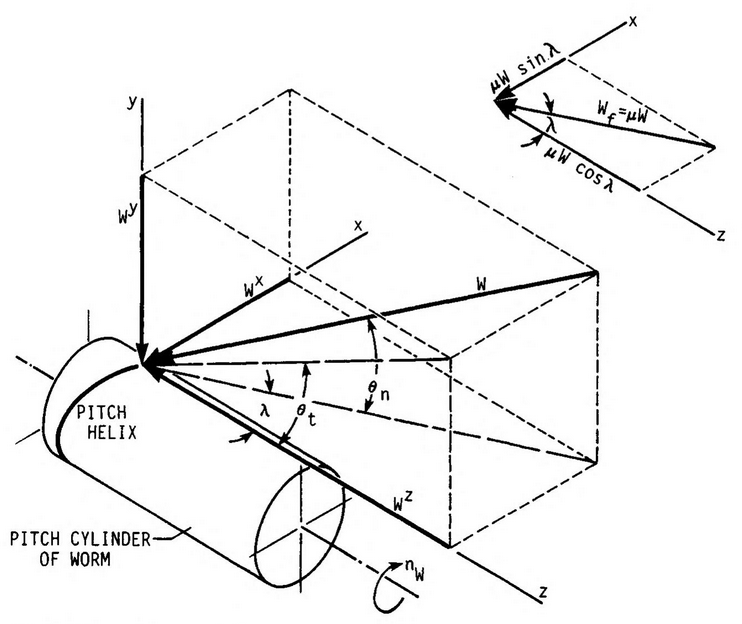
\includegraphics[width=0.6\linewidth]{media/gearFORCE.png}
    \caption{Ανάλυση δυνάμεων στην οδοντοκίνηση ατέρμονα - τροχού \cite{handbook}.}
    \label{fig:gearFORCE}
\end{figure}

Προκύπτει ότι οι συνιστώσες υπολογίζονται ως:
\begin{align}
    W_x &= W \cdot (cos\phi_n sin\lambda + \mu cos\lambda)\\
    W_y &= W \cdot  sin\phi_n \\
    W_z &= W \cdot (cos\phi_n cos\lambda - \mu sin\lambda)
\end{align}

Γίνεται εύκολα αντιληπτό ότι η αξονική φόρτιση των εδράνων είναι η $W_z$ ενώ η ακτινική προκύπτει μέσω των άλλων δύο ως η υποτείνουσα του τριγώνου τους:
\begin{align}
    F_a &= W_z\\
    F_r &= \sqrt{W_x^2 + W_y^2}
\end{align}

Ωστόσο, επειδή οι δυνάμεις δεν ασκούνται στον άξονα της ατράκτου αλλά σε απόσταση $D/2$ από τον κεντρικό της άξονα, θα πρέπει να εισαχθεί και μια διόρθωση λόγω των ροπών που δημιουργούν αυτές οι δυνάμεις ως προς το κέντρο της ατράκτου. Η κάθετη ακτινική δύναμη $W_y$, δε δημιουργεί κάποια ροπή καθώς διέρχεται από το κέντρο της ατράκτου, η εφαπτομενική συνιστώσα $W_x$, δημιουργεί ροπή που τείνει να περιστρέψει την άτρακτο γύρω από τον κεντρικό άξονα της. Τα ρουλεμάν δε αντιστέκονται σε αυτή τη κίνηση. Τέλος, η αξονική δύναμη $W_z$, δημιουργεί ροπή που καταπονεί τα έδρανα ακτινικά. Έτσι, αυτή πρέπει να ληφθεί υπόψη κατά τη διόρθωση των δυνάμεων στις εδράσεις. Επομένως έχουμε τη ροπή που δημιουργεί η αξονική δύναμη:
\begin{equation}
    M_{tip} = W_z \cdot \frac{D}{2}
\end{equation}

Η αντίστοιχη δύναμη διόρθωσης, λόγω της παραπάνω ροπής, στα έδρανα προκύπτει ως η δύναμη που χρειάζεται να προστεθεί στις αντιδράσεις για να ισσοροπήσει το ισοζύιγο δυνάμεων:
\begin{equation}
    F_{corr} = \frac{M_{tip}}{L}
\end{equation}
Όπου $L$, είναι η απόσταση από τα σημεία εφαρμογής των εδράνων κύλισης.
\begin{figure}[H]
    \centering
    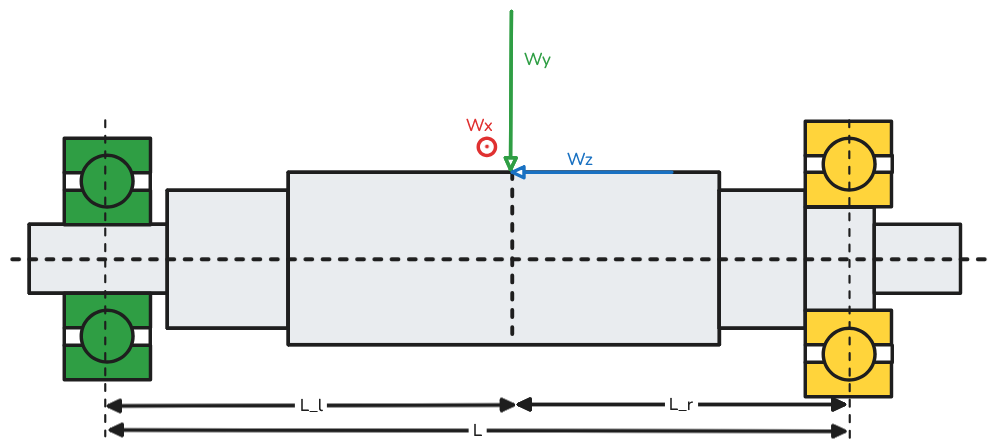
\includegraphics[width=0.6\linewidth]{media/bearForce.png}
    \caption{Ανάλυση δυνάμεων εδράνων κύλισης ατράκτου ατέρμονα.}
    \label{fig:bearForce}
\end{figure}

Η ακτινική δύναμη πρέπει να μοιραστεί και αυτή με βάση την απόσταση των εδράνων από το κέντρο εφαρμογής των δυνάμεων της οδοντοκίνησης. Αυτή αναλύεται ως εξής:
\begin{align}
    F_{r_{l}} &= F_r \cdot \frac{L_r}{L}\\
    F_{r_{r}} &= F_r \cdot \frac{L_l}{L}
\end{align}

Προσθέτωντας και στα δύο έδρανα τη διόρθωση προκύπτει για τη συνολική ανάλυση:
\begin{align}
    F_a &= W_z\\
    F_{r_{l}} &= F_r \cdot \frac{L_r}{L} + F_{corr}\\ 
    F_{r_{r}} &= F_r \cdot \frac{L_l}{L} + F_{corr}
\end{align}

Στη συγκεκριμένη οδοντοκίνηση, ισχύει ότι η αξονική συνιστώσα των δυνάμεων είναι:
\begin{equation}
    W_x = \frac{2\cdot T_M}{D}
\end{equation}

Όπου $T_M$ η ροπή το εκάστοτε κινητήρα όπως φαίνεται στον \ref{tab:motors} και $D$ η διάμετρος λειτουργίας του ατέρμονα κοχλία όπως υπολογίστηκε στον \ref{tab:gearComp}. Έτσι, μπορούν εύκολα να προκύψουν όλες οι συνιστώσες των δυνάμεων της οδοντοκίνησης και κατ' επέκταση των εδράνων κύλισης στον \ref{tab:bearForce} και να επιλυθούν τα έδρανα στο λογισμικό KISSsoft.







\par Επίσης, τα περικόχλια ατράκτου, γίνονται και αυτά εμφανή από τα σκαριφήματα των υποσυστημάτων του συστήματος κίνησης. Όπως αναφέρθηκε αυτά επιλέχθηκαν από τον κατάλογο της McMaster και της MISUMI, όπως αυτά ικανοποιούν τις χωροταξικές απαιτήσεις της κατασκευής. Στον \ref{tab:locknutBOM} φαίνονται τα επιλεγμένα περικόχλια ατράκτου.

\begin{table}[H]
    \centering
    \rowcolors{2}{gray}{white}
\begin{tabular}{|c|c|c|c|c|}
\hline
\rowcolor{Dandelion}
Lock Nut & Catalogue & Usage & Thread $[mm]$ & Lock Type\\
\hline

3552N17 & McMaster-Carr & Fix 61804 bearing & $M14\times1$ & Nylon insert grip \\
\hline
3552N19 & McMaster-Carr & Fix 61903 bearing & $M15\times1$ & Nylon insert grip \\
\hline
BNG4 & MiSUMi & Tighten indirect bearing arrangement & $M4\times1$ & Set screw and pin \\
\hline
BNG6 & MiSUMi & Fix W 607 bearing & $M6\times1$ & Set screw and pin \\
\hline


\end{tabular}

    \caption{Περικόχλια ατράκτου συστήματος κίνησης.}
    \label{tab:locknutBOM}
\end{table}

\par Η πρώτη κατηγορία (τύπου McMaster Nylon Insert) αξιοποιεί τις ελαστικές ιδιότητες των πολυμερών για την επίτευξη αυτοασφάλισης. Τα συγκεκριμένα περικοχλία φέρουν ενσωματωμένο στο εσωτερικό τους έναν δακτύλιο από πολυαμίδιο, ο οποίος έχει εσωτερική διάμετρο ελαφρώς μικρότερη από αυτή του σπειρώματος της ατράκτου. Κατά τη βίδωμα, το σπείρωμα του άξονα εισέρχεται στο νάιλον ένθετο, προκαλώντας του ελαστική και εν μέρει πλαστική παραμόρφωση. Η ελαστική επαναφορά του υλικού ασκεί συνεχή ακτινική πίεση στα σπειρώματα, δημιουργώντας υψηλές δυνάμεις τριβής που αποτρέπουν την ακούσια χαλάρωση λόγω κραδασμών. Το πλεονέκτημα αυτής της μεθόδου είναι η στεγανοποίηση της σύνδεσης και η απορρόφηση των μικρο-δονήσεων, ενώ ταυτόχρονα αποφεύγεται η μεταλλική φθορά στην άτρακτο.

\par Η δεύτερη κατηγορία περικοχλίων (σειρά Misumi BNG) ενσωματώνει έναν μηχανισμό ασφάλισης που βασίζεται στην τριβή, χωρίς όμως να προκαλεί φθορά στο σπείρωμα του άξονα. Κάθε περικόχλιο φέρει στο σώμα του, κάθετα προς τον άξονα περιστροφής, έναν ή περισσότερους κοχλίες ακινητοποίησης (set screws). Η καινοτομία έγκειται στην παρεμβολή ενός μικρού κυλινδρικού παρεμβύσματος,  κατασκευασμένου συνήθως από μαλακότερο μέταλλο, μεταξύ του κοχλία ακινητοποίησης και του σπειρώματος της ατράκτου. Κατά τη σύσφιξη του κοχλία ακινητοποίησης, η πίεση μεταφέρεται στο παρέμβυσμα, το οποίο πιέζει τα σπειρώματα της ατράκτου δημιουργώντας την απαραίτητη δύναμη συγκράτησης. Με αυτόν τον τρόπο επιτυγχάνεται ισχυρή ακινητοποίηση χωρίς ο χαλύβδινος κοχλίας να έρχεται σε άμεση επαφή με την άτρακτο, αποτρέποντας έτσι τον τραυματισμό των σπειρωμάτων

\begin{figure}[H]
    \centering
    \begin{subfigure}{0.45\linewidth}
        \centering
        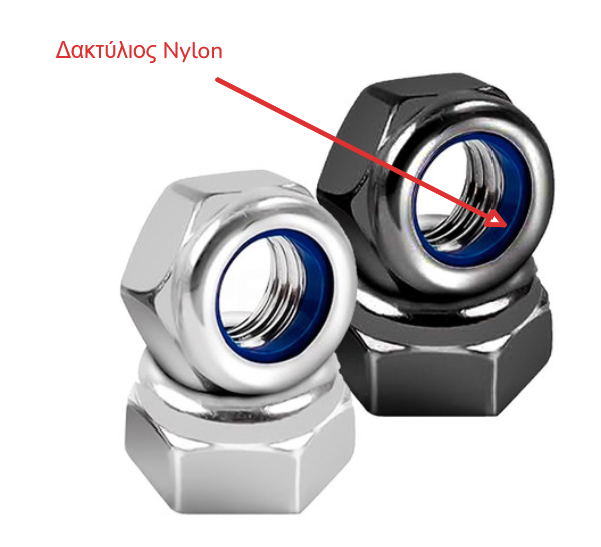
\includegraphics[width=\linewidth]{media/locknut1.png}
        \caption{Ασφάλιση με δακτύλιο πολυαμιδίου.}
        \label{fig:locknut1}
    \end{subfigure}
    \hfill
    \begin{subfigure}{0.45\linewidth}
        \centering
        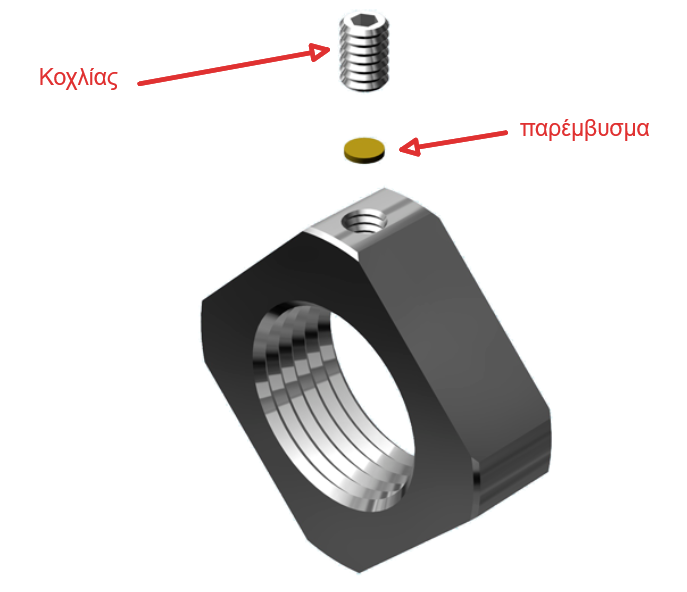
\includegraphics[width=\linewidth]{media/locknut2.png}
        \caption{Ασφάλιση με παρέμβυσμα.}
        \label{fig:locknut2}
    \end{subfigure}
    \caption{Τρόποι ασφάλισης περικοχλίων ατράκτου του συστήματος κίνησης.}
    \label{fig:lockNUTS}
\end{figure}




\section{Ανάλυση στοιχείων με χρήση λογισμικού}
\subsection{Εισαγωγή παραμέτρων και συντελεστές ασφαλείας οδοντοκίνησεων}

Έχοντας υπολογίσει τα γεωμετρικά μεγέθη των οδοντωτών τροχών του συστήματος κίνησης, μπορούν να εισαχθούν οι παραπάνω μεταβλητές στο λογισμικό υπολογισμού αντοχής KISSsoft για υπολογισμό χεύγους ατέρμονα - τροχού (Worms with enveloping worm wheels). Αρχικά, στρογγυλοποιείται το αξονικό μέτρο οδόντωσης της οδοντοκίνησης της ερπύστριας σε $m_x = 1.65\; mm$. Έπειτα εισάγονται οι παράκτω παράμετροι ως δεδομένα στους πίνακες υπολογισμού:
\begin{itemize}
    \item Αξονικό μέτρο οδόντωσης $m_x$.
    \item Δόντια ατέρμονα και τροχού $z_1, z_2$.
    \item Γωνία πίεσης $\phi_n$.
\end{itemize}

Μέσω των παραπάνω, και ορίζοντας την αξονική απόσταση των γραναζιών προκύπτουν αυτόματα η γωνίας ελίκωσης του ατέρμονα $\lambda$. Στη συνέχεια, υπολογίζονται τα πλάτη των γραναζιών ακολουθώντας τους τύπους του Niemann. Με βάση αυτούς προκύπτει αυτόματα από το λογισμικό ότι το μέγιστο πλάτος του ατέρμονα για την ερπύστρια δε πρέπει να ξεπερνάει τα $f \le 44.6\; mm$. Επομένως, σύμφωνα με τους αναλυτικούς υπολογισμούς, θα πρέπει να ισχύει $48.41 \ge f \le 44.6$, το οποίο είναι αδύνατο. Έτσι, ορίζεται το πλάτος του ατέρμονα για την ερπύστρια ώστε να ικανοποιεί τις προϋποθέσεις του Niemann με βάση το λογισμικό. Κρατώντας όλες τις υπόλοιπες μεταβλητές στις τυπικές τιμές του (defaul settings), προκύπτουν ποιότητες με βάση το DIN 3974, 6 και 7 για τον ατέρμονα και τον τροχό αντίστοιχα. Τα προφίλ των οδοντώσεων επιλέγονται τυπικά με βάση το ISO 53: Type C, από τις διαθέσιμες επιλογές του λογισμικού. Ενώ οι ανοχές επιλέγονται και αυτές αυτόματα. Τέλος, ορίζεται το ποσοστό του χρόνου χρήσης της οδοντοκίνησης στα $100\%$, κάτι που δεν ισχύει στη πραγματικότητα, για την μελέτη του δυσμενέστερου σεναρίου για τα γρανάζια. Εισάγωντας και τις αποστάσεις των εδράνων κύλισης από το κέντρο του ατέρμονα, όπως αυτές έχουν προκύψει από τον προκαταρκτικό σχεδιασμό, υπολογίζονται από το λογισμικό τα παρακάτω:
\begin{itemize}
    \item Διάρκεια ζωής οδοντοκίνησης $H$.
    \item Διάμετρος λειτουργίας ατέρμονα και τροχού $d_m = D_i,\; i = W or i = G$.
    \item Συντελεστής ασφαλείας σε εκκοιλάνσεις $S_H$.
    \item Συντελεστής ασφαλείας σε θραύση $S_F$.
    \item Συντελεστής ασφαλείας σε φθορά $S_W$.
    \item Θερμοκρασιακός συντελεστής ασφαλείας $S_T$.
    \item Συντελεστής ασφαλείας έναντι βέλους κάμψης του άξονα ατέρμονα $S_\delta$.
\end{itemize}

Παρακάτω παρατίθονται τα υπολογιστικά επιλυόμενα γεωμετρικά χαρακτηριστικά των οδοντώσεων όπως προκύπτουν μέσω του λογισμικού αλλά και οι συντελεστές ασφαλείας των οδοντοκινήσεων. Να σημειωθεί ότι τα υλικά επιλέγονται ως έχουν κατά τη δεύτερη επανάληψη του ισοζυγίου μάζας (Steel για τον ατέρμονα και Aluminum για το γρανάζι). Ο συγκεκριμένος κωδικός υλικού επιλέγεται από τις διαθέσιμες επιλογές του λογισμικού ώστε να προκύπτουν ικανοποιητικοί συντελεστές ασφαλείας. Αντίστοιχα επιλέγεται και η λίπανση για τη κάθε οδοντοκίνηση. Οι υπολογισμοί γίνονται με βάση το DIN 3996:2019.
\begin{table}[H]
    \centering
    \rowcolors{2}{gray}{white}
\begin{tabular}{|c|c|r|r|}
\hline
\rowcolor{YellowGreen}
Characteristic & Units & TRACKS & FLIPPER \\
\hline
$\lambda$ & $^\circ$ &  7.96 & 7.59\\ 
\hline
$m_x$ & $mm$ &  1.65 & 2.00\\ 
\hline
$r_c$ & $mm$ &  4.25 & 5.50\\ 
\hline
$f$ & $mm$ &  40 & 40\\ 
\hline
$F_e$ & $mm$ &  11.2 & 15.0\\ 
\hline
$D_{a,2}$ & $mm$ &  51.5 & 56.0\\ 
\hline
$D_W$ & $mm$ &  11.8 & 15.0\\ 
\hline
$D_G$ & $mm$ &  46.2 & 50.0\\ 
\hline
Worm Material & $-$ &  \multicolumn{2}{c|}{X46Cr13} \\ 
\hline
Gear Material & $-$ &  \multicolumn{2}{c|}{2024-T4}\\ 
\hline
Lubrication Method & $-$ &  \multicolumn{2}{c|}{Injection}\\ 
\hline
Lubricant & $-$ &  \multicolumn{2}{c|}{Kluberoil 4UH1-32N}\\ 
\hline
\end{tabular}
    \caption{Υπολογιστικά αποτελέσματα οδοντοκινήσεων ερπύστριας και βραχίονα.}
    \label{tab:gearComp}
\end{table}

\par Όπως παρατηρείται, μεταξύ αναλυτικών και υπολογιστικών αποτελεσμάτων υπάρχουν κάποιες διαφορές στα γεωμετρικά μεγέθη. Να σημειωθεί ότι τα μεγέθη του \ref{tab:gearComp} προκύπτουν έπειτα από κάποιες επαναλήψεις με κύριο γνώμονα οι συντελεστές ασφαλείας να προκύπτουν $S \ge 1.1$. Τα νούμερα που δίνονται είναι τα τελικά υπολογιζόμενα ώστε να ικανοποιείται αυτός ο περιορισμός. Ο συντελεστής της εφαρμογής $K_A$ επιλέγεται ως $K_A = 1.75$ για την ερπύστρια και ως $K_A = 1.6$ για τον βραχίονα, σύμφωνα με το DIN 3990/ISO 6336.
\begin{figure}[H]
    \centering
    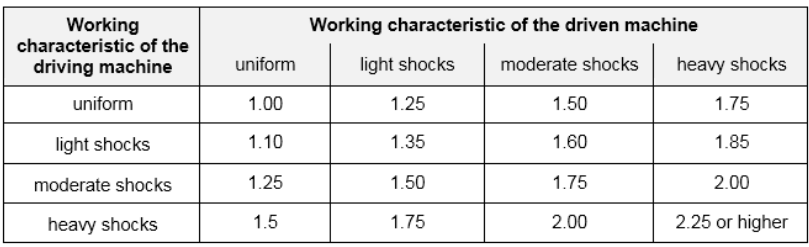
\includegraphics[width=0.6\linewidth]{media/KA.png}
    \caption{Συντελεστής εφαρμογής σύμφωνα με το DIN 3990/ISO 6336.}
    \label{fig:KA}
\end{figure}


Ορίζοντας ως στόχο χρόνου λειτουργίας τις 20000 ώρες για την οδοντοκίνηση προκύπτουν οι συντελεστές ασφαλείας της πλατφόρμας. Η τιμή αυτή εκλέχθηκε με βάση μια τυπική διάρκεια αποστολής έρευνας (4 ώρες). Επομένως, με στόχο τις \textbf{5000 αποστολές} έως την ανάγκη αλλαγής των γραναζιών προκύπτει ο χρόνος λειτουργίας.


\begin{table}[H]
    \centering
    \rowcolors{2}{gray}{white}
\begin{tabular}{|c|r|r|}
\hline
\rowcolor{Dandelion}
Safety Factor & TRACKS & FLIPPER \\
\hline
$S_F$ &  4.892 & 14.580\\ 
\hline
$S_H$ &  1.164 & 1.838\\ 
\hline
$S_W$  &  999.900 & 999.900\\ 
\hline
$S_T$  &  13.350 & 26.703\\ 
\hline
$S_\delta$  &  1.402 & 5.658\\ 
\hline

\end{tabular}

    \caption{Συντελεστές ασφαλείας για χρόνο λειτουργίας της πλατφόρμας $H = 20000\;h$.}
    \label{tab:sf}
\end{table}



Η μέγιστη διάρκεια ζωής προκύπτει όταν ο συντελεστής ασφαλείας σε εκκοιλάνσεις (ο μικρότερος από όλους) παίρνει την τιμή της μονάδας. Αυτό συμβαίνει για χρόνο λειτουργίας $H_{max} = 49796$ για την ερπύστρια και $H_{max} = 770391$ για τον βραχίονα, υποθέτοντας όπως αναφέρθηκε διάρκεια χρησιμοποίησης της οδοντοκίνησης $100\%$.

\par Επίσης, ο συντελεστής φθοράς όπως φαίνεται υπολογίζεται και στις δύο περιπτώσεις 999.90. Αυτός δεν είναι ο πραγματικός συντελεστής όσο ένα όριο του ίδιου του λογισμικού, υπονοώντας ότι ο ρυθμός φθοράς είναι σχεδόν μηδενικός. Αυτό συμβαίνει λόγω της φαινομενικά μικρής ροπής επί των γραναζιών και κατ' επέκταση της μικρής επιφανειακής πίεσης των δοντιών. 

\par Παρακάτω, προκύπτει από το λογισμικό KISSsoft, η τρισδιάστατη απεικόνιση (μοντέλο CAD) των δύο οδοντοκινήσεων. Δηλαδή η πλήρης και ορθά ορισμένη γεωμετρία των γραναζιών για την επίτευξη των στόχων ζωής της πλατφόρμας.
\begin{figure}[H]
    \centering
    \begin{subfigure}{0.45\linewidth}
        \centering
        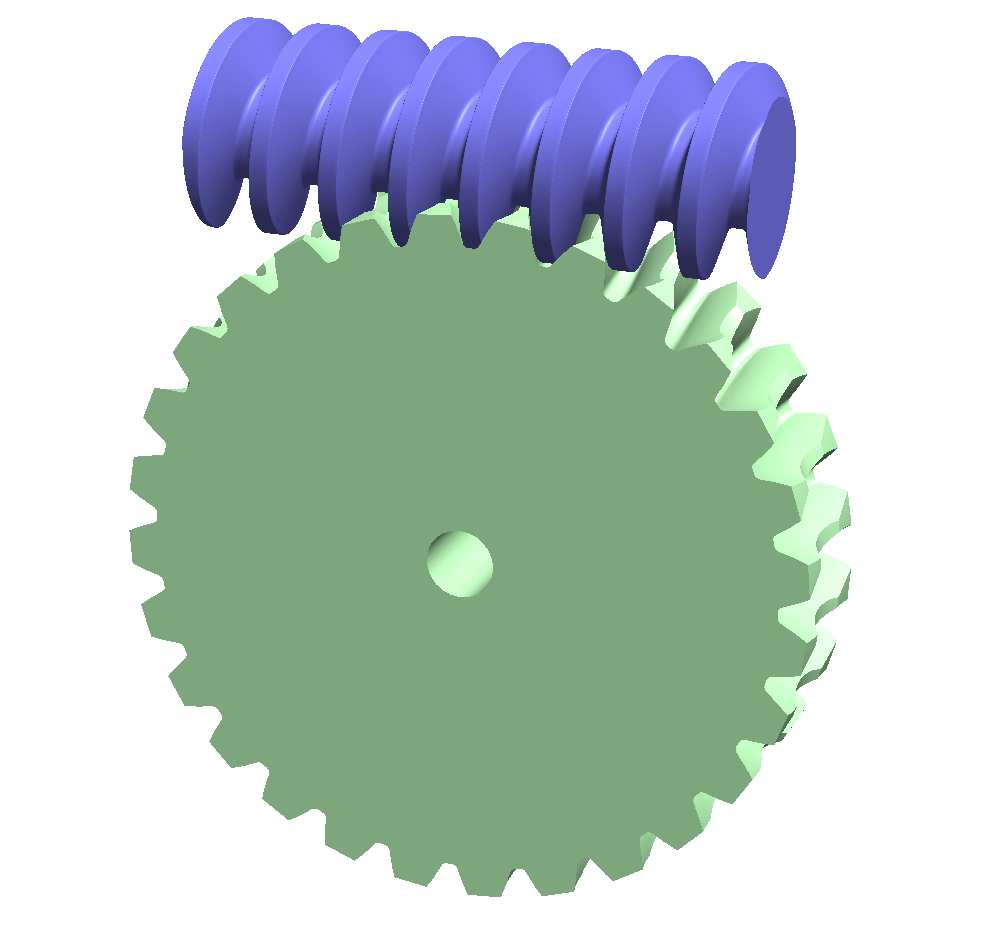
\includegraphics[width=\linewidth]{media/tracksKISSSOFT.png}
        \caption{Ερπύστριας.}
        \label{fig:tracksKISSSOFT}
    \end{subfigure}
    \hfill
    \begin{subfigure}{0.45\linewidth}
        \centering
        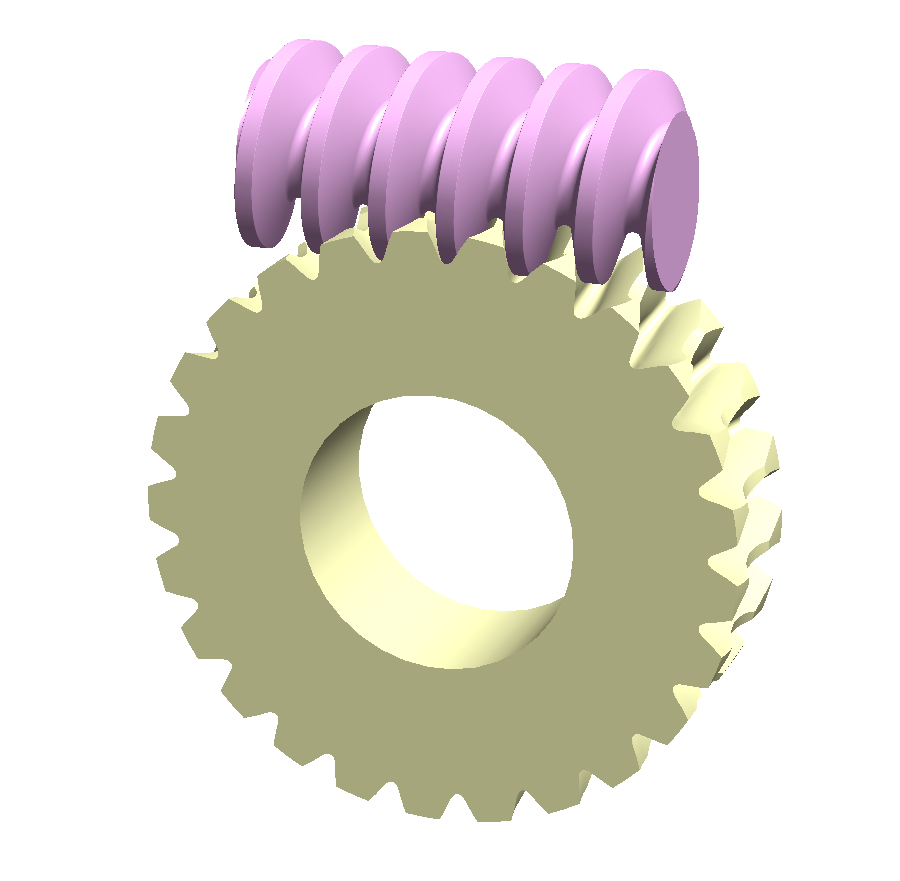
\includegraphics[width=\linewidth]{media/flipperKISSSOFT.png}
        \caption{Βραχίονα.}
        \label{fig:flipperKISSSOFT}
    \end{subfigure}
    \caption{τρισδιάστατα μοντέλα CAD οδοντωτών ζεύγων ατέρμονα - τροχού για την ερπύστρια και τον περιστρεφόμενο βραχίονα της πλατφόρμας.}
    \label{fig:kisssoftGEARS}
\end{figure}





\subsection{Εισαγωγή παραμέτρων και συντελεστές ασφαλείας εδράσεων}


Όπως αναφέρθηκε και παραπάνω, έχουν γίνει οι υπολογισμοί των δυνάμεων που καταπονούν τα έδρανα κύλισης της ατράκτου του ατέρμονα. Αυτές προκύπτουν από τις δυνάμεις που αναπτύσσονται στα δόντια των γραναζιών και της ροπής του ηλεκτροκινητήρα που τα κινεί.


\begin{table}[H]
    \centering
    \rowcolors{2}{gray}{white}
\begin{tabular}{|c|r|r|r|}
\hline
\rowcolor{Dandelion}
Force $[N]$ & $F_a$ & $F_{r_{l}}$& $F_{r_{r}}$ \\
\hline

TRACKS & 314 & 91 & 97 \\
\hline

FLIPPER & 198 & 62 & 63 \\
\hline



\end{tabular}

    \caption{Δυνάμεις καταπόνησης εδράνων κύλισης ατράκτου ατέρμονα.}
    \label{tab:bearForce}
\end{table}





Εισάγωντας λοιπόν τα παρακάτω στο λογισμικό KISSsoft:
\begin{itemize}
    \item Περιστροφική ταχύτητα κινητήρα $n_M\; [rpm]$.
    \item Αξονική δύναμη καταπόνησης $F_a\; [N]$.
    \item Ακτινική δύναμη καταπόνησης για κάθε έδρανο $F_r\; [N]$.
    \item Τα επιλεγμένα έδρανα W 636 και W 607 ως κινητό και πακτωμένο αντίστοιχα.
\end{itemize}

Υπολογίζονται αυτόματα οι χρόνοι λειτουργίας των εδράνων $L_{10h}$ στον \ref{tab:L10h}.

\begin{table}[H]
    \centering
    \rowcolors{2}{gray}{white}
\begin{tabular}{|c|c|r|r|}
\hline
\rowcolor{YellowGreen}
$L_{10h}\; [h]$ & W 636 & W 607\\
\hline
TRACKS & 38992 & 267\\
\hline
FLIPPER & 140947 & 1004\\
\hline
\end{tabular}
    \caption{Χρόνος λειτουργίας εδράνων κύλισης ατράκτου ατέρμονα.}
    \label{tab:L10h}
\end{table}



Παρατηρώντας το μιρκότερο χρόνο λειτουργίας με εμπιστευτικότητα $90\%$ στις $267\; h$, ορίζεται και ο πραγματικός χρόνος λειτουργίας στις $260\;h$ για να προκύψουν και οι συντελεστές ασφαλείας της κατασκευής.

\begin{table}[H]
    \centering
    \rowcolors{2}{gray}{white}
\begin{tabular}{|c|c|r|r|}
\hline
\rowcolor{YellowGreen}
$S_0$ & W 636 & W 607\\
\hline
TRACKS & 8.571 & 2.718\\
\hline
FLIPPER & 12.581 & 4.276\\
\hline
\end{tabular}
    \caption{Συντελεστές ασφαλείας εδράνων κύλισης ατράκτου ατέρμονα για 260 ώρες λειτουργίας με εμπιστευτικότητα $90\%$.}
    \label{tab:s0}
\end{table}



Όπως παρατηρείται, οι χρόνοι λειτουργίας είναι αρκετά ικανοποιητικοί. Μετά από 260 ώρες λειτουργίας της πλατφόρμας ή όπως αναφέρθηκε (για 4 ώρες διάρκεια αποστολής διάσωσης) για 65 αποστολές, κρίνεται αναγκαία η αλλαγή των εδράνων κύλισης που επιλέχθηκαν. Διαφορετικά μπορούν αν επιλεχθούν και έδρανα με μεγαλύτερη στατική και δυναμική αντοχή για την επέκταση της διάρκειας ζωής της πλατφόρμας.

\section{Επικοινωνία χειριστή με την πλατφόρμα}

Η αμφίδρομη επικοινωνία μεταξύ του ρομποτικού διασώστη και του Σταθμού Ελέγχου Εδάφους (Ground Control Station - GCS) υλοποιείται μέσω ασύρματου τοπικού δικτύου WLAN. Συγκεκριμένα, η κεντρική υπολογιστική μονάδα της πλατφόρμας (Raspberry Pi 5) διαμορφώνεται ώστε να λειτουργεί ως Ασύρματο Σημείο Πρόσβασης (Wireless Access Point / Hotspot), δημιουργώντας ένα αυτόνομο δίκτυο στο οποίο συνδέεται ο φορητός υπολογιστής του χειριστή, ο οποίος φέρει λειτουργικό σύστημα Linux. Αυτή η τοπολογία εξασφαλίζει τη δυνατότητα επικοινωνίας ακόμα και σε περιβάλλοντα όπου δεν υφίσταται προϋπάρχουσα δικτυακή υποδομή, συνθήκη τυπική για αποστολές έρευνας και διάσωσης USAR.

\par Η ανταλλαγή δεδομένων βασίζεται στο λογισμικό μεσαίου επιπέδου ROS (Robot Operating System), το οποίο ακολουθεί την αρχιτεκτονική Publisher-Subscriber. Η ροή της πληροφορίας διακρίνεται σε δύο σκέλη:

\begin{enumerate}
\item \textbf{Τηλεμετρία και Λήψη Δεδομένων (Upstream Flow)}. Όσον αφορά την εποπτεία της κατάστασης του ρομπότ, οι επιμέρους κόμβοι λογισμικού (ROS nodes) που εκτελούνται στο Raspberry Pi είναι υπεύθυνοι για την ανάγνωση των αισθητήρων. Τα δεδομένα αυτά (εικόνα κάμερας, νέφος σημείων LiDAR, δεδομένα αδράνειας IMU, μετρήσεις αερίων) δημοσιεύονται σε πραγματικό χρόνο σε συγκεκριμένα θεματικά κανάλια (topics), όπως για παράδειγμα \/camera\/image\_raw, \/scan και \/imu/data. Ο σταθμός ελέγχου, δηλαδή το laptop, λειτουργώντας ως συνδρομητής (subscriber) σε αυτά τα κανάλια, λαμβάνει τα πακέτα δεδομένων και τα οπτικοποιεί μέσω γραφικού περιβάλλοντος (ROS GUI tools, όπως το RViz ή το rqt), παρέχοντας στον χειριστή πλήρη εικόνα του πεδίου επιχειρήσεων.

\item \textbf{Τηλεχειρισμός και Έλεγχος Κίνησης (Downstream Flow)}. Για τις περιπτώσεις που απαιτείται χειροκίνητη παρέμβαση, ο χειριστής έχει τη δυνατότητα ανάληψης του ελέγχου μέσω ασύρματου χειριστηρίου (gamepad). Η διαδικασία ελέγχου ακολουθεί την εξής αλληλουχία: 
\begin{itemize} 
    \item Ένας κόμβος στον υπολογιστή του χειριστή (π.χ. \texttt{joy\_node}) αναγιγνώσκει τις εντολές από τα πλήκτρα και τους αναλογικούς μοχλούς και τις δημοσιεύει στο κανάλι \/joy. 
    \item Στη συνέχεια, ένας ενδιάμεσος κόμβος μετατροπής (π.χ. \texttt{teleop\_twist\_joy}) μεταφράζει τις εντολές αυτές σε κινηματικά μεγέθη (γραμμική και γωνιακή ταχύτητα) και τις δημοσιεύει στο κεντρικό κανάλι ελέγχου κίνησης \/cmd\_vel. 
    \item Τέλος, ο ελεγκτής των κινητήρων (motor controller) που εκτελείται στο ρομπότ, εγγράφεται στο κανάλι \/cmd\_vel, λαμβάνει τις επιθυμητές ταχύτητες και τις μετατρέπει στα κατάλληλα σήματα PWM για την οδήγηση των κινητήρων. 
\end{itemize}

\end{enumerate}

\begin{figure}[H]
    \centering
    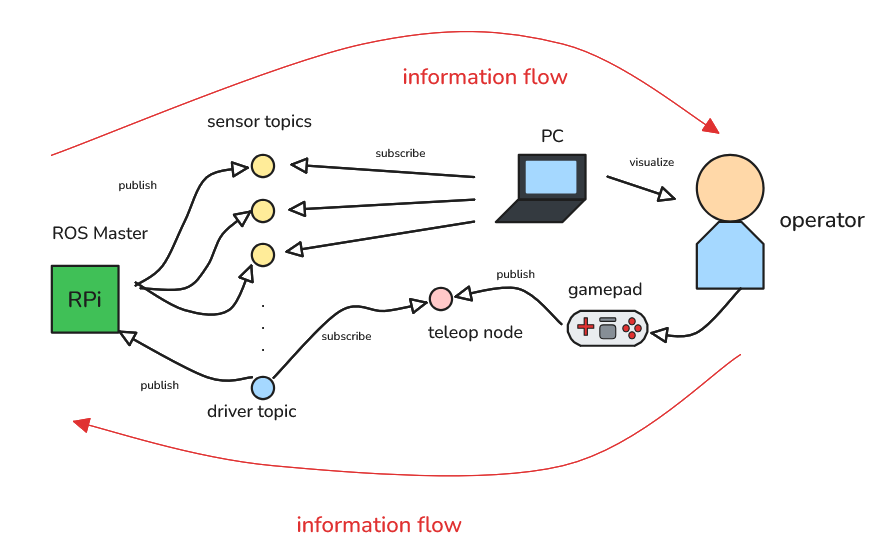
\includegraphics[width=0.6\linewidth]{media/ros.png}
    \caption{Ροή πληροφορίας μεταξύ πλατφόρμας V.L.A.D. και χειριστή.}
    \label{fig:ros}
\end{figure}